\chapter{Operations \& Logistics}
\setlength{\parindent}{15pt}
\label{ch:oper_logi}

\section{Operations \& Logistics Concept Description}
\label{sec:oper_logi_conc_desc}

\begin{figure}[htb]
    \centering
    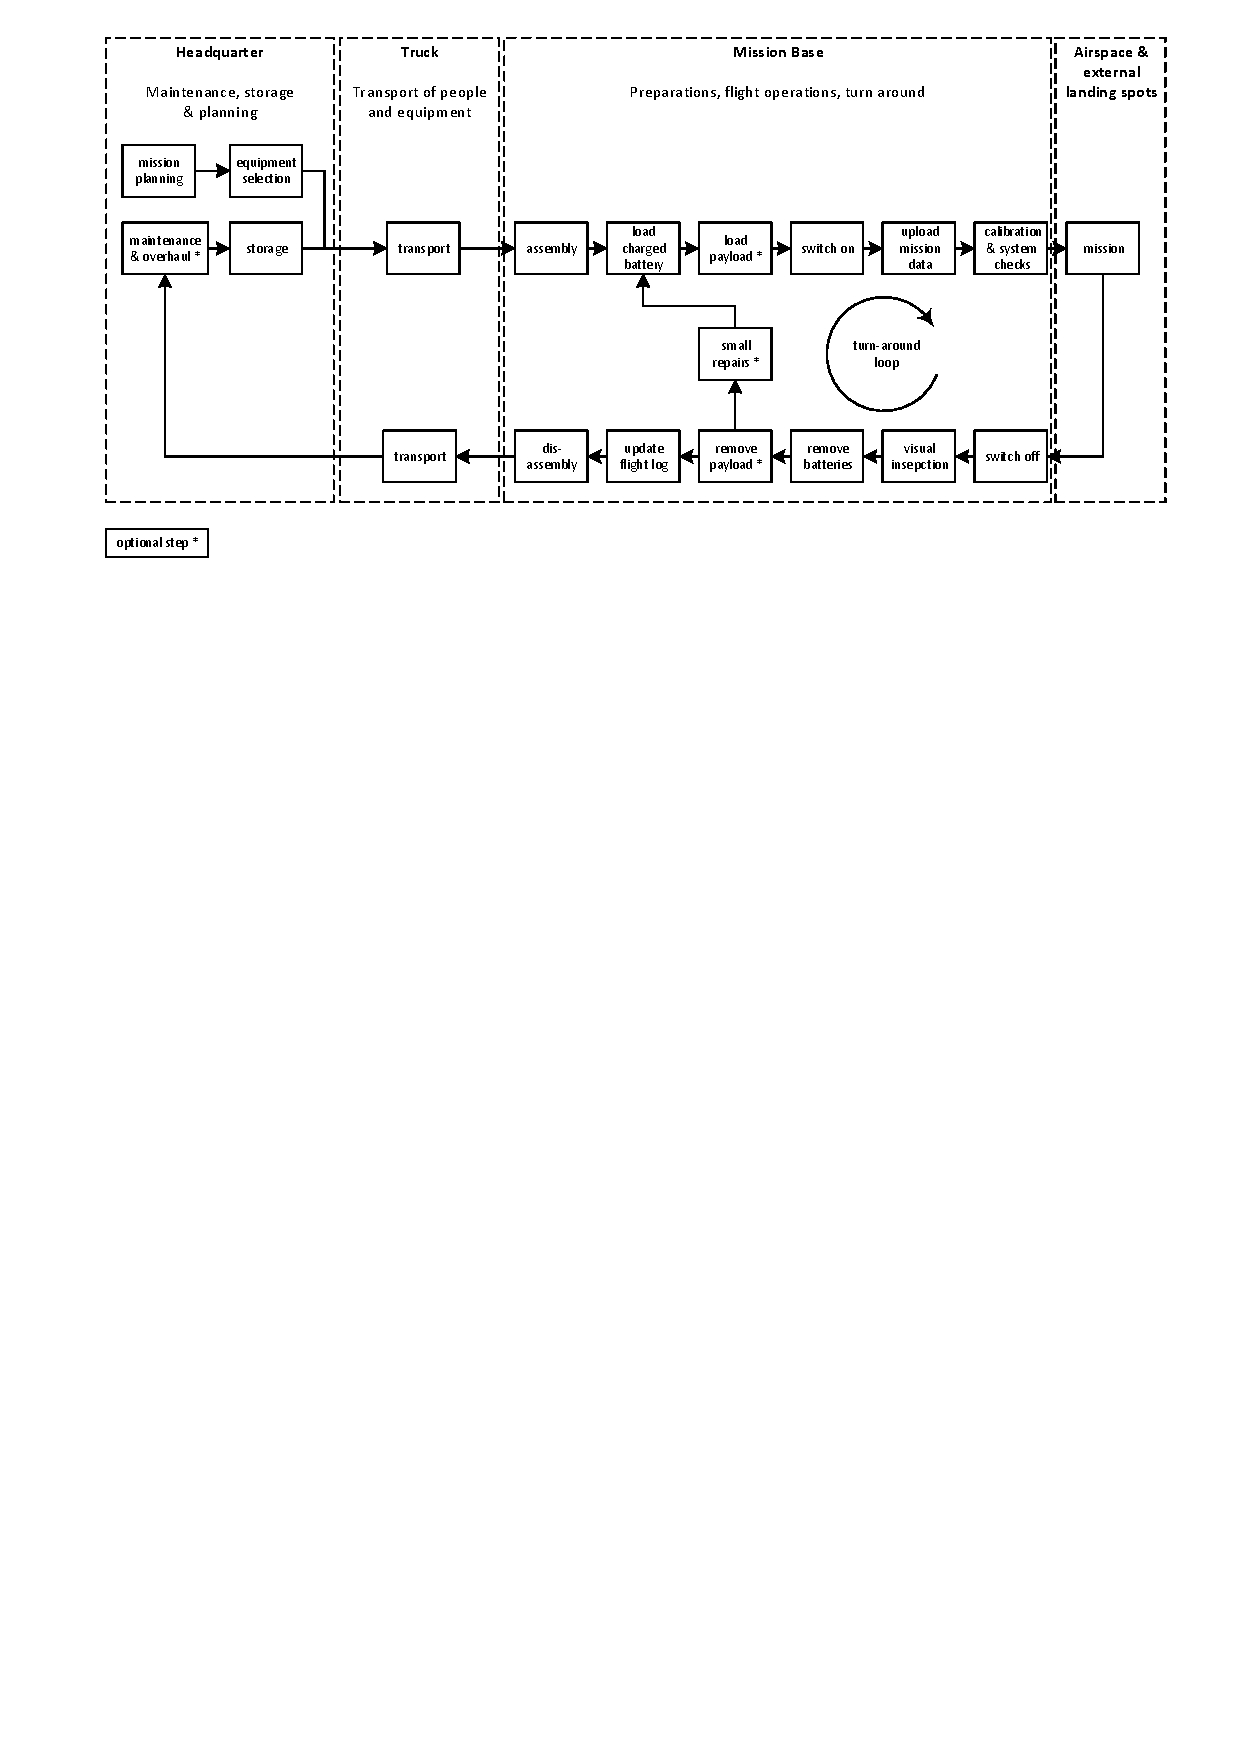
\includegraphics[width=1\textwidth]{OperationsLogistics/Figures/operations_logistics.pdf}
    \caption{Operations \& Logistics Flow Diagram}
    \label{fig:opslogsdig}
\end{figure}

\autoref{fig:opslogsdig} shows the the operations and logistics flow diagram for what this group expects to be typical operating conditions. It is assumed that the UAV operator has a main facility, from which the UAV, staff and mission relevant equipment are transported to a mission base at which flight operations take place. Naturally, variations to this scheme are possible, e.g. a parcel company may exclusively operate from its main facility, or long-range missions require a turn-around at a remote location, but for the sake of brevity only the most general case is presented.
The starting and end point of each mission is the so-called headquarters, the place where maintenance and storage takes place. Based on customer input a mission plan is set up, which determines the kind of resources that are required. Next to one or more UAVs, this includes staff on site, equipment such as the ground station, spare parts, additional batteries and a transport vehicle. Once the preparation is done, everything is loaded into a vehicle and transported to the location where the UAV is intended to take off and land. On site, the equipment needs to be unloaded and the UAV assembled into its operational form. A charged battery is then loaded, followed by the payload, which can also consist of another set of batteries. The system is switched on, the mission relevant data is uploaded to the on-board computer and an automated instrument calibration and readiness check performed. The UAV is now ready to fly and carry out its mission. After its return, the system is switched off for safety reasons, visually inspected and stripped off its batteries. The next steps depend on the kind of mission in question. If another flight is scheduled, the payload can be replaced and minor repairs taken out, e.g. replacing a damaged propeller blade. Once the battery is recharged or replaced by a full one, a new flight cycle can start. In case the mission does not comprise a turn-around or substantial damage was detected, the digital flight log is updated and the UAV disassembled. After loading all equipment the transport back to the headquarter takes place, where scheduled maintenance and all levels of repairs are carried out. Once the work is documented and approved, the equipment is stored and ready for the next mission.

\section{RAMS Characteristics}
\label{sec:rams_char}

